\documentclass{beamer}
\usepackage{amsfonts,amsmath,oldgerm}
\usepackage[nameinlink]{cleveref}
\usepackage[dvipsnames]{xcolor}
\usepackage{graphicx}
\usepackage{hyperref}
\usepackage[
    backend=biber,
    style=alphabetic,
    sorting=anyt,
    minnames=3,
    minalphanames=3
]{biblatex}

\hypersetup{
    colorlinks=true,
    citecolor=red,
    linkcolor=white,
    urlcolor=black,
    pdftitle={NA Seminar},
}
    
\usetheme{sintef}

\definecolor{Carmine}{HTML}{9e0e24}

\newcommand{\N}{\mathbb{N}}                     % Natural Numbers
\newcommand{\rbk}[1]{\left(#1\right)}
\newcommand{\curlyquotes}[1]{\textquotedblleft #1\textquotedblright}
\newcommand{\boldred}[1]{\textcolor{Carmine}{\textbf{#1}}}
\DeclareMathOperator*{\argmax}{\mathrm{argmax}}    % Expected value
    
\usefonttheme[onlymath]{serif}
\setbeamercovered{transparent}
    
\titlebackground*{assets/background}

\title{Application of reinforcement learning \\to medium access control for
WSNs}
\subtitle{Autonomous Networking}
\course{Master's Degree in Computer Science}
\author{\href{https://github.com/Exyss/}{Simone Bianco}}
\IDnumber{1986936}
\date{Academic Year 2025/2026}

\addbibresource{../references.bib}

\begin{document}
\maketitle


% \begin{frame}

% This template is a based on \hrefcol{https://www.overleaf.com/latex/templates/sintef-presentation/jhbhdffczpnx}{SINTEF Presentation} from \hrefcol{mailto:federico.zenith@sintef.no}{Federico Zenith} and its derivation \hrefcol{https://github.com/TOB-KNPOB/Beamer-LaTeX-Themes}{Beamer-LaTeX-Themes} from Liu Qilong

% \vspace{\baselineskip}

% In the following you find a brief introduction on how to use \LaTeX\ and the beamer package to prepare slides, based on the one written by \hrefcol{mailto:federico.zenith@sintef.no}{Federico Zenith} for \hrefcol{https://www.overleaf.com/latex/templates/sintef-presentation/jhbhdffczpnx}{SINTEF Presentation}

% % This template is released under \hrefcol{https://creativecommons.org/licenses/by-nc/4.0/legalcode}{Creative Commons CC BY 4.0} license

% \end{frame}

\section{Introduction}

\begin{frame}{Introduction}
\framesubtitle{Wireless Sensor Networks}

    \begin{columns}
        \begin{column}{0.5\textwidth}
            
            \boldred{Wireless Sensor Network (WSN)} are networks composed by distributed sensing devices used to monitor and record environmental conditions and events.

            \uncover<+->{
                \begin{itemize}[<+->]
                    \item Low-cost sensors
                    \item Large number of nodes
                    \item Multi-hop wireless communication
                    \item Sink nodes on the edge of the network
                \end{itemize}
            }
        \end{column}

        \begin{column}{0.5\textwidth}
            \begin{figure}[H]
                \centering
                \includegraphics[scale=0.2]{../images/wsn.png}
            \end{figure}
        \end{column}
    \end{columns}
\end{frame}

\begin{frame}{Benefits}
\framesubtitle{Wireless Sensor Networks}

    WSNs are employed \boldred{\textit{everywhere}} there is a need for monitoring a physical space or using sensors for controlling a procedure.
    
    \uncover<+->{
        \begin{itemize}[<+->]
            \item Simplicity
            \item Large-scale coverage
            \item Autonomous operations
            \item High scalability
            \item Real-time data
        \end{itemize}
    }
\end{frame}

\begin{frame}{Issues}
\framesubtitle{Wireless Sensor Networks}
    
    \uncover<+->{
        \curlyquotes{All that glisters is not gold!}
        \begin{flushright}
        - The Merchant of Venice, William Shakespeare
        \end{flushright}

        \quad
    }
    
    \uncover<+->{
        Due to their nature, WSNs suffer from \boldred{critical} issues.
        \begin{itemize}[<+->]
            \item Limited computation power
            \item Asymmetric flow of information
            \item \boldred{Energy consumption}
        \end{itemize}
    }
\end{frame}

\begin{frame}{Any solutions?}
\framesubtitle{Wireless Sensor Networks}
    
    \uncover<+->{
        Many protocols have been proposed to mitigate these issues.
        \begin{itemize}
            \item S-MAC, Z-MAC, \dots
        \end{itemize}
    }

    \uncover<+->{
        Some protocols even achieve great results, but they are too \boldred{complex}.
        \begin{itemize}
            \item Quorum-MAC (Q-MAC), Low-Energy Adaptive Clustering Hierarchy (LEACH), \dots
        \end{itemize}
    }

    
    \uncover<+->{
        \qquad

        \boldred{New idea}: Reinforcement Learning $\to$ Introducing \boldred{Aloha-Q}!
    }
\end{frame}

\section{The Aloha-Q protocol}

\begin{frame}{The main idea}
\framesubtitle{The Aloha-Q protocol}
    
    \uncover<+->{
        Framed Slotted Aloha (FSA) with stateless \boldred{Q-Learning}. 
        \begin{itemize}
            \item Learn from collisions!
        \end{itemize}
    }

    \begin{figure}
        \centering
        \includegraphics[scale=0.6]{../images/slotted_2.pdf}
    \end{figure}
\end{frame}


\begin{frame}{The main idea}
\framesubtitle{The Aloha-Q protocol}
    
    \begin{itemize}[<+->]
        \item \textit{Frame size} $M$ is approximately (and at least) equal to the number $N$ of nodes
        \item Each node has individual \boldred{Q values} for every slot in the frame 
        \begin{itemize}
            \item Values are updated after each transmission
            \item The largest value determines which slot is selected for the next transmission
        \end{itemize}
        \item \boldred{Acknowledgement (ACK)} messages are sent when a message is received
        \item Nodes \boldred{wake up} only when they need to transmit and to receive ACKs
        \begin{itemize}
            \item Synchronization times are embedded in ACK messages
        \end{itemize}
        \item Only the sink nodes use \textit{idle listening}
    \end{itemize}
\end{frame}

\begin{frame}{Learning scheme}
\framesubtitle{The Aloha-Q protocol}
    
    \begin{itemize}[<+->]
        \item Each node acts as an agent based on the \boldred{K-Armed Bandit}
        \begin{itemize}
            \item State space: $\mathcal{S} = \{0\}$
            \item Action space: $\mathcal{A} = \{0, \ldots, M-1\}$
        \end{itemize}
        \item When the scheme converges, each node has an associated slot (recall $M \geq N$)
        \item Q values are described by a function $Q(x,k)$, where $x$ is the node and $k$ is the slot
        \item Each node $x$ transmits in the slot $k^*$ with the \boldred{highest Q value} for the node itself.
        $$k^* \in \argmax\limits_{k \in \mathcal{A}} Q(x,k)$$
    \end{itemize}
\end{frame}

\begin{frame}{K-Armed Bandit}
\framesubtitle{The Aloha-Q protocol}
    
    \begin{itemize}[<+->]
        \item Each node starts with all Q values set to $0$
        \begin{itemize}
            \item \boldred{Optimistic randomized start}
        \end{itemize}
        \item When a node $x$ transmits in slot $k$, the Q value is updated:
        $$Q_{t+1}(x,k) \gets Q_t(x,k) + \alpha(r-Q_t(x,k))$$

        where $\alpha \in [0,1]$ is the \textit{learning rate} and $r$ is the \textit{reward}
    \end{itemize}
\end{frame}

\begin{frame}{K-Armed Bandit}
\framesubtitle{The Aloha-Q protocol}
    
    \begin{itemize}[<+->]
        \item $\alpha$ controls the \textit{convergence speed}
        \begin{itemize}
            \item Usually set to $\alpha = 0.1$ to mitigate node failures
        \end{itemize}
        \item A reward $r = +1$ is given for \boldred{successes}, while $r = -1$ is given for \boldred{collisions}
        \begin{itemize}
            \item Collisions are highly punished when the Q value is positive
            \item Successes are highly rewarded when the Q value is negative
        \end{itemize}
    \end{itemize}

    \begin{figure}
        \centering
        \includegraphics[scale=0.5]{../images/qvalues.png}
    \end{figure}
\end{frame}

\section{Convergence of Aloha-Q}

\begin{frame}{Assumptions}
\framesubtitle{Convergence of Aloha-Q}
    \begin{itemize}[<+->]
        \item Single-hop networks with $N$ nodes and saturated traffic conditions
        \item Frame size equal to $N$
        \item Each node may trasmit only one packet per frame
        \item Learning rate set to $\alpha = 1$
        $$Q_{t+1}(x,k) \gets Q_t(x,k) + 1 \cdot (r-Q_t(x,k)) = r$$
    \end{itemize}
\end{frame}

\begin{frame}{Definitions}
\framesubtitle{Convergence of Aloha-Q}
    \begin{itemize}[<+->]
        \item \boldred{Steady node}: a node with Q values set to $-1$ for all slots except for one set to $+1$
        \begin{itemize}
            \item Otherwise, \textit{hopping node}
        \end{itemize}
        \item \boldred{Occupied slot}: a slot with Q values set to $-1$ for all nodes except for one set to $+1$
        \begin{itemize}
            \item Otherwise, \textit{unoccupied node}
        \end{itemize}
    \end{itemize}
\end{frame}


\begin{frame}{Markov model}
\framesubtitle{Convergence of Aloha-Q}
    We consider a \boldred{Markov chain} with state space $\mathcal{I} = \{0, \ldots, N\}$
    \begin{itemize}[<+->]
        \item Each state $i \in \mathcal{I}$ represents the number of steady nodes/occupied slots
        \item For each state $i \in \mathcal{I}-\{0,N\}$ we define three transitions: $p_{i,i}, p_{i,i-1}$ and $p_{i,i+1}$.
        \item State $0$ has only two transitions: $p_{0,0}$ and $p_{0,1}$ 
        \item State $N$ has only one transition: $p_{N,N}$ 
    \end{itemize}

    \begin{figure}[H]
        \centering

        \resizebox{1\textwidth}{!}{
            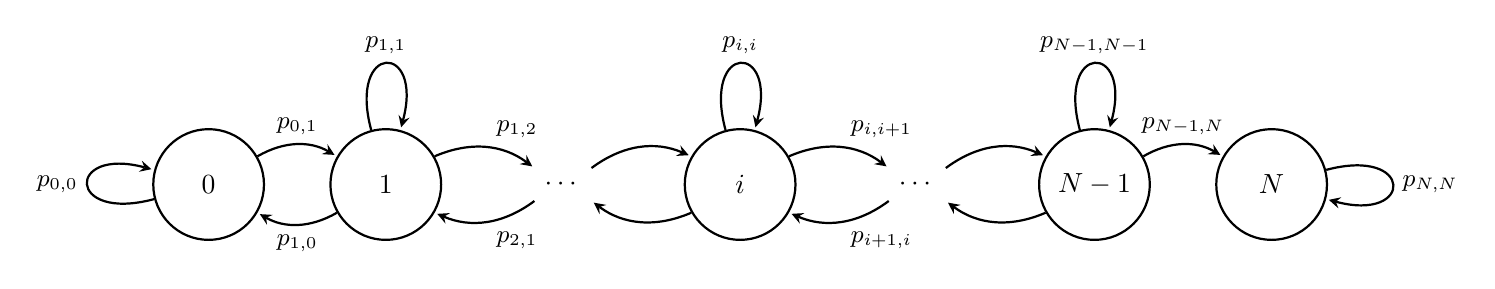
\begin{tikzpicture}[->,>=stealth,shorten >=1pt,auto,node distance=2.25cm,thick,main node/.style={scale=0.8, circle,draw,font=\sffamily\normalsize}]

                \node[circle, draw, minimum size = 40] (0) []{$0$};
                \node[circle, draw, minimum size = 40] (1) [right of = 0]{$1$};
                \node[]      (x) [right of = 1]{$\cdots$};
                \node[circle, draw, minimum size = 40] (2) [right of = x]{$i$};
                \node[]      (y) [right of = 2]{$\cdots$};
                \node[circle, draw, minimum size = 40] (3) [right of = y]{$N-1$};
                \node[circle, draw, minimum size = 40] (4) [right of = 3]{$N$};

                \path[every node/.style={font=\sffamily\small}]
                    (0) edge[loop left] node{$p_{0,0}$} (0)
                    (0) edge[bend left] node{$p_{0,1}$} (1)

                    (1) edge[loop above] node{$p_{1,1}$} (1)
                    (1) edge[bend left] node{$p_{1,2}$} (x)
                    (1) edge[bend left] node{$p_{1,0}$} (0)

                    (x) edge[bend left] (2)
                    (x) edge[bend left] node{$p_{2,1}$} (1)

                    (2) edge[loop above] node{$p_{i,i}$} (2)
                    (2) edge[bend left] node{$p_{i,i+1}$} (y)
                    (2) edge[bend left] (x)

                    (y) edge[bend left] (3)
                    (y) edge[bend left] node{$p_{i+1,i}$} (2)

                    (3) edge[loop above] node{$p_{N-1,N-1}$} (3)
                    (3) edge[bend left] node{$p_{N-1, N}$} (4)
                    (3) edge[bend left] (y)

                    (4) edge[loop right] node{$p_{N,N}$} (4)
                ;
            \end{tikzpicture}
        }
    \end{figure}
\end{frame}


\begin{frame}{Markov model}
\framesubtitle{Convergence of Aloha-Q}
    
    We move \boldred{up one state} when the current slot is unoccupied and only one hopping node transmits in it
    $$p_{i,i+1} = \underbrace{\rbk{\frac{N-i}{N}}}_{\text{Pr. of unoccupied slot}} \cdot \underbrace{\rbk{\frac{N-i}{N}} \rbk{\frac{N-1}{N}}^{N-i-1}}_{\text{Pr. of $=1$ hopping node when unoccupied}}$$

\end{frame}

\begin{frame}{Markov model}
\framesubtitle{Convergence of Aloha-Q}
    
    We move \boldred{down one state} when the current slot is occupied and one or more hopping nodes transmits in it
    $$p_{i,i-1} = \underbrace{\rbk{\frac{i}{N}}}_{\text{Pr. of occupied slot}} \cdot \underbrace{\rbk{1-\rbk{\frac{N-1}{N}}^{N-i}}}_{\text{Pr. of $\geq 1$ hopping nodes when occupied}}$$
\end{frame}

\begin{frame}{Markov model}
\framesubtitle{Convergence of Aloha-Q}
    
    We stay in the \boldred{same state} when:
    \begin{itemize}
        \item The current slot is occupied and no hopping nodes select the current slot.
        \item The current slot is unoccupied and two or more hopping nodes transmit packets in it.
        \item The current slot is unoccupied and there are no transmissions in it.
    \end{itemize}

    $$p_{i,i} = \frac{i}{N} \rbk{\frac{N-1}{N}}^{N-i} + \frac{N-i}{N}\rbk{1-\frac{N-i}{N} \rbk{\frac{N-1}{N}}^{N-i-1}}$$
\end{frame}

\begin{frame}{Limiting distribution}
\framesubtitle{Convergence of Aloha-Q}
    
    Convergence is achieved when $\lim\limits_{n \to +\infty} P^n_{i,N} = 1$ for all $i \in \{0, \ldots, N\}$
    \begin{itemize}
        \item $P$ is the \boldred{Probability Transition Matrix (PTM)} of the Markov chain
        \item $P_{i,j}^n = \sum\limits_{m = 0}^N P^{n-1}_{i,m} P_{m,j}$
    \end{itemize}

    \quad
    
    \quad

    It can be proven that the above \boldred{limiting distribution} converges
\end{frame}


\begin{frame}{Expected convergence time}
\framesubtitle{Convergence of Aloha-Q}
    
    Expected number of visits to all states, except state $N$, across all $n$ steps as $n \to +\infty$, starting from state $0$.

    $$\mathbb{E}[T] = \sum_{n = 1}^{+\infty} \sum_{j = 0}^{N-1} P^n_{0,j}$$

    Requires intensive computations due to no closed form
\end{frame}


\section{Performance of Aloha-Q}

\begin{frame}{Simulations}
\framesubtitle{Performance of Aloha-Q}
    
    $100-200$ simulations, $50-100$ practical trials, various network sizes

    \begin{figure}[H]
        \centering
        \begin{tabular}{ll}
            \hline
            Parameters & Values \\
            \hline
            Channel bit rate & 250 kbits/s \\
            Data packet length (simulation) & 1044 bits \\
            Data packet length (practical) & 935 bits \\
            ACK packet length (simulation) & 20 bits \\
            ACK packet length (practical) & 144 bits \\
            Slot length & 1100 bits \\
            \hline
        \end{tabular}
    \end{figure}
\end{frame}

\begin{frame}{Convergence time}
\framesubtitle{Performance of Aloha-Q}
    
    \begin{figure}[H]
        \centering
        \includegraphics[scale=0.41]{../images/conv_time.png}
        \includegraphics[scale=0.4]{../images/cdf_conv_time.png}
    \end{figure}
\end{frame}

\begin{frame}{Throughput}
\framesubtitle{Performance of Aloha-Q}
    
    \begin{figure}[H]
        \centering
        \includegraphics[scale=0.5]{../images/throughput.png}
    \end{figure}
\end{frame}

\begin{frame}{Delay and Energy consumption}
\framesubtitle{Performance of Aloha-Q}
    
    \begin{figure}[H]
        \centering
        \includegraphics[scale=0.4]{../images/delay.png}
        \includegraphics[scale=0.45]{../images/energy.png}
    \end{figure}
\end{frame}

\begin{frame}{Conclusions}
\framesubtitle{Performance of Aloha-Q}
    
    Summary of \boldred{Aloha-Q} performance analysis:
    \begin{itemize}
        \item Simulations and practical trials are close to theoretical limits
        \item Convergence is reached in short time (relative to lifespan of the WSN)
        \item Performance is better than S-MAC and very close to Z-MAC (when converged)
        \item Way less over overhead than already existing protocols
    \end{itemize}

\end{frame}

\backmatter[notitle]
    
% \begin{frame}{Bibliography}
% \framesubtitle{{}}
%     \printbibliography
% \end{frame}

\end{document}
